% !TeX spellcheck = nl_BE
\documentclass{article}
\usepackage{hyperref}
\usepackage{graphicx}
\usepackage{listings}
\newcommand{\HRule}{\rule{\linewidth}{0.5mm}}
\newcommand{\thedate}{2 Juni 2014}
\newcommand{\projectname}{ProgrammeerProject 2}
\title{Codeverslag Programmeerproject 2}
\author{Arno De Witte\\
Vrije Universiteit Brussel}
\date{2 Juni 2014}
\begin{document}


\begin{titlepage}
\begin{center}


\includegraphics[width=0.60\textwidth]{./VUB_logo_compact.jpg}~\\[1cm]


\textsc{\Large Programmeerproject 2}\\[0.5cm]

% Title
\HRule \\[0.4cm]
{ \huge \bfseries Codeverslag}\\[0.4cm]

\HRule \\[1.5cm]

% Author and supervisor
\begin{minipage}{0.4\textwidth}
\begin{flushleft} \large
Arno \textsc{De Witte}\\
\end{flushleft}
\end{minipage}
\begin{minipage}{0.5\textwidth}
\begin{flushright} \large
\emph{Titularis:}\\ Prof. Dr. Theo D’Hondt\\
\emph{Assistenten:}\\ Kevin Van Vaerenbergh\\
Lode Hoste\\
Yves Vandriessche
\end{flushright}
\end{minipage}

\vfill

% Bottom of the page
{\large \thedate}

\end{center}
\end{titlepage}

%\maketitle
\newpage
\tableofcontents
\newpage


\section{Inleiding}\label{inleiding}
In dit document kan er een handleiding voor gebruikers en een handleiding voor ontwikkelaars gevonden worden. De handleiding voor gebruikers bevat een overzicht van hoe je het systeem moet gebruiken. De handleiding voor ontwikkelaars bespreekt elk onderdeel van de code uitvoerig.\\
Het systeem draagt de naam Control Your House omdat je ermee heel je huis kan bedienen van achter je computer. Verder is het systeem geschreven in het Engels. Zowel de code, commentaar maar ook de interface. De handleiding in dit document is wel in het Nederlands.\\
De code is meegeleverd in hetzelfde archief als waarin dit document kan worden gevonden en is voornamelijk geschreven in Racket, met onderdelen in slip en R5RS.\\
Het doel van dit project is om een domotica systeem te schrijven. Dit systeem bestaat uit 3 delen. Een majordomo: dit is een computer die heel het systeem beheert, een steward: dit zijn kleine computers (bijvoorbeeld een raspberry pi) die commando's krijgen over een lokaal netwerk en deze dan doorsturen naar de devices. De devices zijn het laatste deel, dit zijn slimme apparaten die via het Zigbee protocol verschillende boodschappen (messages) verstaan. Ze kunnen deze uitvoeren en een antwoord terugsturen.\\

\section{Handleiding voor gebruikers}
\label{sec:users}
In dit deel zal er worden uitgelegd hoe je het systeem gebruikt. Er is een opsomming van de functies\ref{sub:features}, hoe het systeem ge\"{i}nstalleerd moet worden\ref{sub:install} en hoe alle functies gebruikt kunnen worden\ref{sub:usage}.

\subsection{Functies}
\label{sub:features}
\begin{itemize}
\item Een simpele, overzichtelijke web interface die kan worden bekeken op alle toestellen die over een browser beschikken en binnen hetzelfde netwerk zitten.
\item Overzicht van alle stewards, met een actuele status. Deze toont aan wanneer bepaalde stewards offline zijn (niet verbonden met netwerk) of hoeveel devices er geconnecteerd zijn aan een bepaalde steward.
\item Mogelijkheid om nieuwe stewards toe te voegen. Je hoeft enkel het ip adres, de poort en de plaats van de steward mee te geven.
\item Automatisch opsporen van devices door de steward. Deze worden getoond in het device overzicht.
\item Bekijken van de actuele status van een device.
\item Rechtstreeks commando's sturen naar devices via het device overzicht. 
\item Ondersteuning voor 2 type devices: ZBS-110 (plug) en ZBS-121 (multimeter).
\item Ophalen van data in de achtergrond. Deze data is wat de verschillende devices als metingen teruggeven.
\item Overzicht waar je de opgehaalde data kan bekijken. Dit kan per kamer of over heel het systeem. Er kunnen waarden worden weggefilterd en er kan voor bepaalde tijdsperioden worden gekozen.
\item Zelf toevoegen van acties. Dit zijn regels die zelf kunnen worden samengesteld. Voor meer uitleg, zie gebruik\ref{sub:actions}.
\item Staat van het systeem wordt persistent opgeslagen. Devices, stewards, acties en data worden veilig opgeslagen. Moest het systeem falen, kan het bij opnieuw opstarten direct hervatten.
\item Stewards en majordomo overleven wanneer de connectie wegvalt. Deze zullen wachten tot er een nieuwe connectie kan worden opgesteld.
\item Mogelijkheid tot simuleren van stewards om te testen.
\end{itemize}
% subsection features (end)

\subsection{Installeren}
\label{sub:install}

Om het systeem te installeren is niet gebruik gemaakt van het racket packaging systeem omdat er verschillende files nodig zijn die niet gemakkelijk te packagen vallen. Ook is de hieronder beschreven methode geldig voor alle besturing systemen.
\begin{enumerate}
	\item Installeer Racket\footnote{http://download.racket-lang.org}. Het systeem is getest onder versie 6.0.
	\item Pak de code uit naar een bepaalde map.
	\item Open DrRacket, open het bestand \emph{start.rkt} en druk rechtsboven op \emph{Doen!}. 
	\item[3b.] Moest het systeem niet snel genoeg lopen, kan in mac en linux via de commandline het commando \lstinline|racket start.rkt| worden uitgevoerd vanaf de map waarin de code zich bevindt. 
	\item Een browser venster opent zich normaal met de interface. Indien dit niet het geval is kan er in een browser naar\\ \emph{http://localhost:8000/servlets/standalone.rkt} worden gesurft.
\end{enumerate}

Om stewards te installeren moet het volgende worden gedaan.
\begin{enumerate}
	\item Kopi\"eer de code in de map \emph{Raspberry} naar de raspberry pi.
	\item Start via Televisie of scherm: 
	\begin{enumerate}
		\item Verbind je raspberry pi met een televisie of scherm. Zet hem aan.
		\item Connecteer de zigbee module.
		\item Login en ga via het cd (change directory) commando naar de map waarin je de inhoud van de map \emph{Raspberry} uit het archief hebt gekopi\"eerd.
		\item Om het ip adres te vinden, druk je het commando \emph{ifconfig} onder eth0 (bekabeld) of wlan0 (wireless), het adres achter "inet addr:" is het ip adres van je steward. De standaard poort is 12345.
		\item Voer het commando \emph{./slip} uit.
		\item Nu moet je de code inladen, dit doe je door \emph{(load "run")} te typen en enter te drukken. 
		\item Je mag de pi nu loskoppelen van het scherm.
	\end{enumerate}
	\item Start de pi via een draadloze ssh verbinding:
	\begin{enumerate}
		\item Sluit de pi aan en connecteer de zibee module.
		\item Het opstellen van de ssh connectie doe je door op je computer \emph{ssh pi@IPVANPI} in te geven.
		\item Hierna zijn stappen e tot g van punt 2 dezelfde.
	\end{enumerate}
	\item Voeg de nieuwe steward toe, door in de interface \emph{Stewards} te drukken. Onderaan de tabel kan je een nieuwe steward toevoegen.
\end{enumerate}
% subsection install (end)

\subsection{Gebruik}
\label{sub:usage}
Het gebruik van het systeem is vrij simpel. Wanneer het systeem wordt opgestart, wordt het start scherm weergegeven. Hierop is er een kleine uitleg over het gebruik van het systeem te vinden. In het menu staan, buiten de startpagina,  4 onderdelen. Deze worden elk hieronder uitgebreid besproken. \\

Op de pagina Stewards kan er een tabel met alle stewards die geconnecteerd zijn aan het systeem gevonden worden. Het ID is de manier waarop het systeem een steward identificeert. Het ip is het lokaal adres waarop de steward zich bevindt. Verder kan je de poort ook zien, deze is standaard 12345. De room is de kamer waarin de steward zich bevindt. Deze moet worden meegegeven bij het toevoegen vermits een raspberry pi onmogelijk zelf kan weten waar hij zich bevindt. Er kan ook de status van de steward worden gevonden. Deze staat in de kolom Amount of devices. Normaal toont deze hoeveel devices er verbonden zijn. Maar wanneer er een netwerk probleem is, of de steward is aan het opstarten zal er een status bericht worden weergegeven (bijvoorbeeld "OFFLINE" wanneer de steward onbereikbaar is).\\
Er kan ook een steward worden toegevoegd. Dit wordt gedaan door in de laatste kolom van de tabel de nodige informatie in te geven in de juiste kolom. Het systeem voegt deze steward dan toe en zal zelf mogelijke devices in de kamer zoeken.\\

De pagina Devices toont een tabel met alle slimme toestellen die ondersteunt worden (voorlopig enkel ZBS-110 en ZBS-121). Er kan verschillende informatie over elk toestel worden gelezen. Alsook een status bericht, dit toont in welke staat het toestel zich bevindt. Bij de ZBS-110 (plug) bijvoorbeeld zal er komen wat de werklast is en of het toestel aan staat of niet. \\
Het is ook mogelijk om rechtstreeks naar het toestel een bericht te sturen. Dit kan in de laatste kolom van de tabel. Merk wel op dat dit een tijdje kan duren, het systeem moet namelijk eerst de berichten die in de achtergrond worden verstuurt afronden en erna het gegeven bericht sturen. Het sturen van een bericht duurt gebruikelijk 10 seconden. Nadat het bericht is verstuurt verschijnt het resultaat in dezelfde kolom als waar het bericht is ingegeven. Merk op dat het systeem zelf toestellen detecteert en deze dus niet handmatig kunnen worden toegevoegd. Het instoppen van toestellen is voldoende.\\

Op de Actions pagina kunnen de acties worden beheert. Een actie bestaat uit een conditie, wanneer deze conditie waar is zal een bepaalde actie worden uitgevoerd. Elke actie heeft een source device, dit is een toestel waaruit de informatie voor de conditie wordt gelezen. De conditie bestaat uit een type, bij temperatuur is dit bijvoorbeeld "TEM"\footnote{Alle types kunnen worden teruggevonden bij de status van toestellen}. Er moet ook een waarde worden meegegeven (bijvoorbeeld 20, van $20\,^{\circ}\mathrm{C}$) en een gelijkheid (bijvoorbeeld kleiner dan).\\
Om de actie iets te laten uitvoeren met je een doeltoestel kiezen en een commando ingeven. Dit commando zal dan naar het toestel worden gestuurd wanneer de conditie waar is.\\
Een uitgewerkt voorbeeld: De elektrische verwarming (aangesloten op een slimme plug) moet worden aangezet wanneer de temperatuur onder de 15 graden zakt. Het type is TEM van temperatuur. De waarde is 15, het doeltoestel is de plug waarin de elektrische verwarming zit, het brontoestel (source device) is de multimeter die te temperatuur in de kamer meet en gelijkheid is kleiner dan ($<$).\\
Acties kunnen worden bekeken, verwijderd en toegevoegd op deze pagina.\\

De laatste pagina is de data pagina. De data die wordt verzameld zijn de status berichten van de verschillende devices, deze worden verzameld in de achtergrond door de majordomo. Op deze pagina staat een korte intro over de data, een lijst met alle kamers waarin er data is verzameld, een link naar de grafiek met alle verzamelde data en een paar feiten over het systeem. Wanneer er wordt verder gegaan naar de data over bijvoorbeeld de badkamer, wordt er een grafiek weergegeven voor de data die in die kamer is verzameld. Er kunnen verschillende data types worden weggelaten en andere tijdsperiodes gekozen. Wanneer er bijvoorbeeld voor minuten wordt gekozen wordt de data van de laatste minuten getoond. Hetzelfde voor dagen enzovoort.\\
% subsection usage (end)


\subsection{Screenshots}
\label{sub:screenshots}
\begin{figure}[htp]
\centering
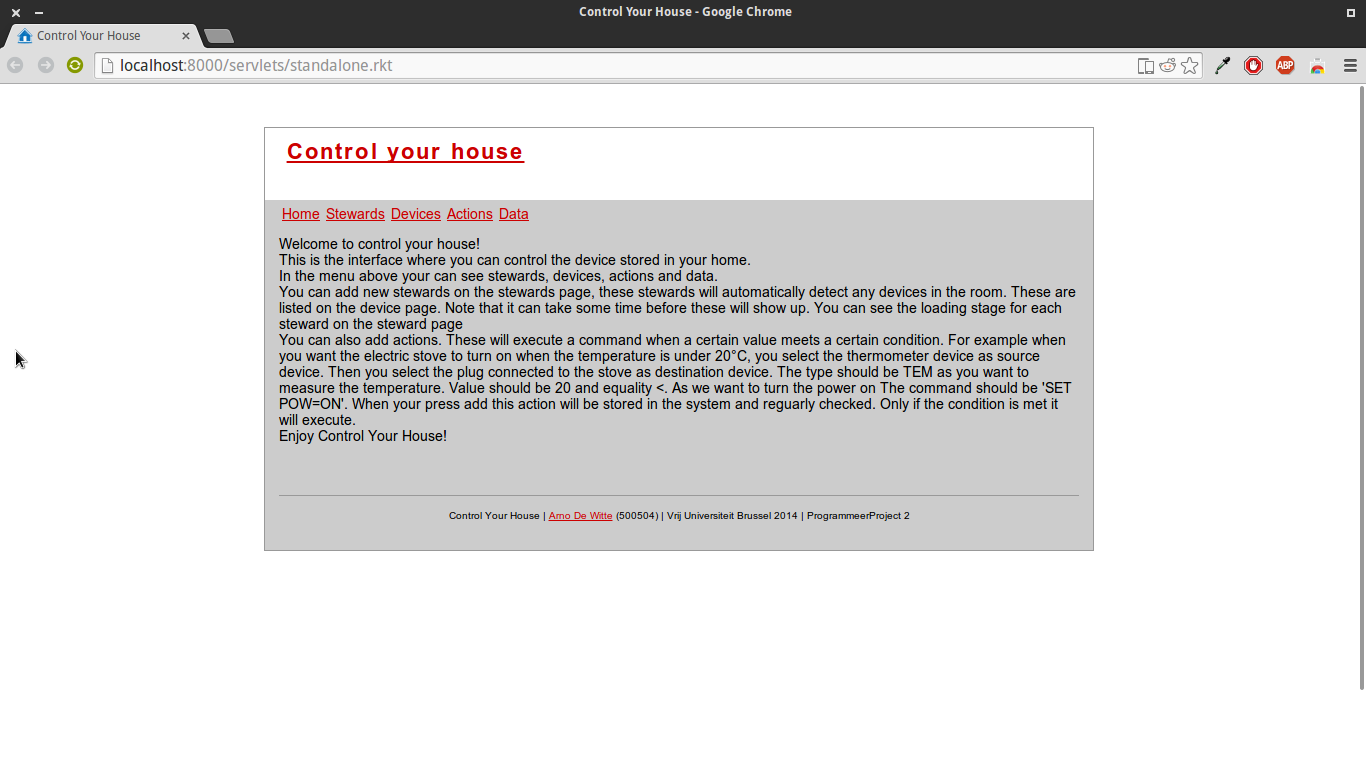
\includegraphics[scale=0.30]{Screenshot1.png}
\caption{Startscherm}
\label{screen1}
\end{figure}
\begin{figure}[htp]
\centering
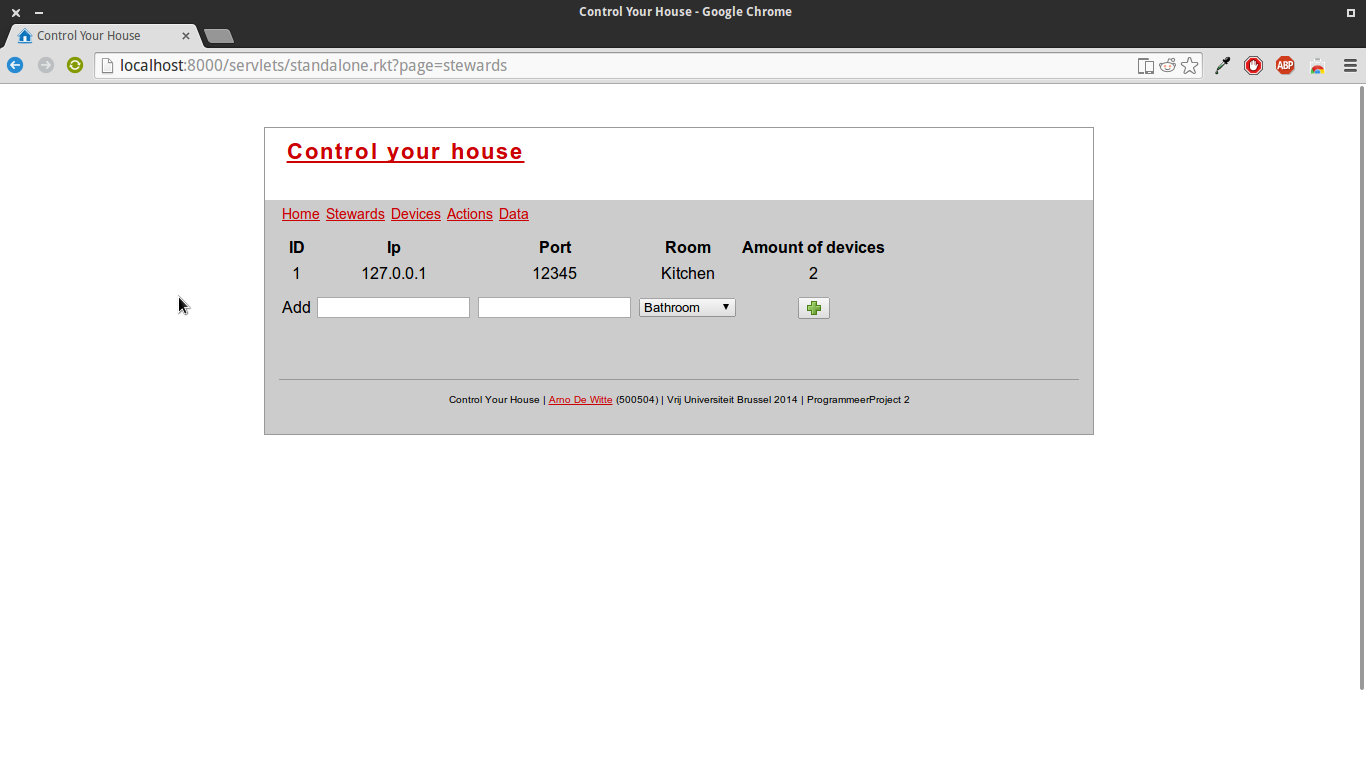
\includegraphics[scale=0.30]{Screenshot2.png}
\caption{Steward scherm}
\label{screen2}
\end{figure}
\begin{figure}[htp]
\centering
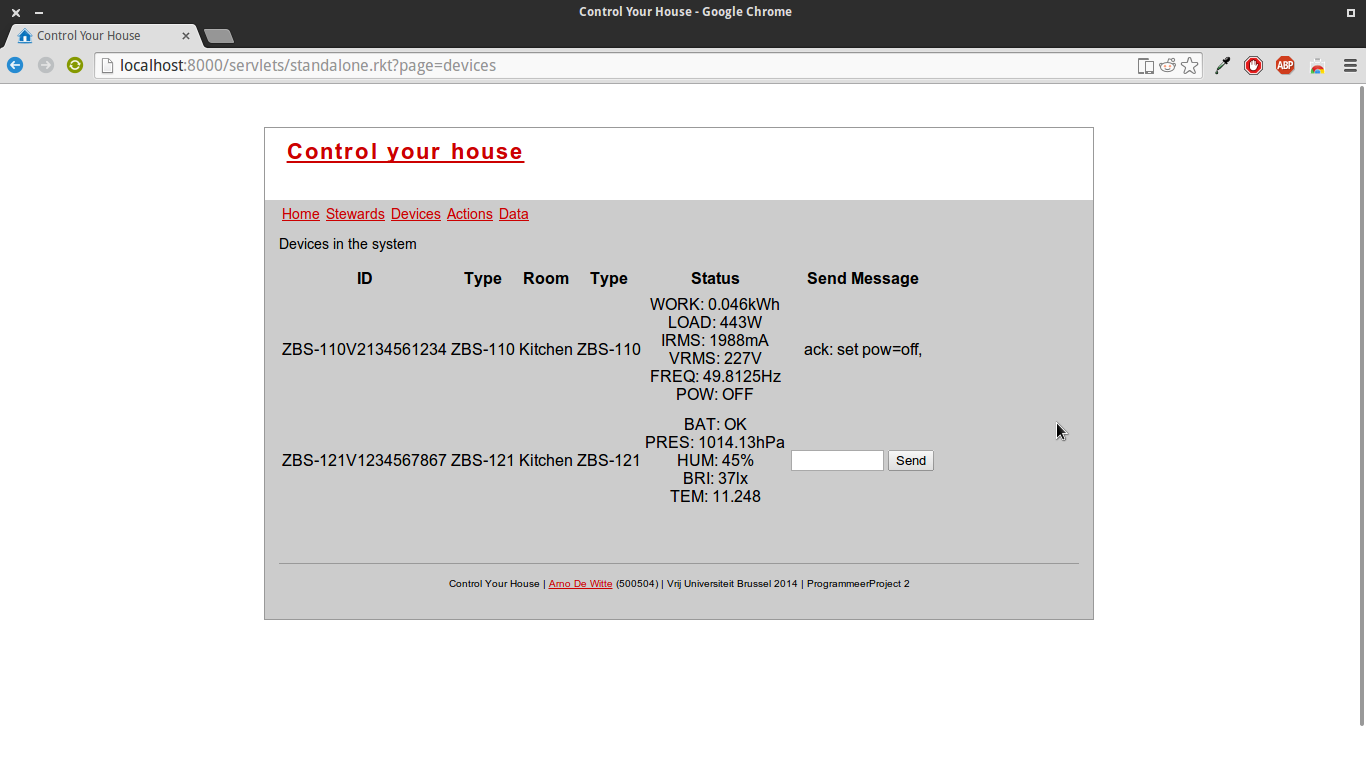
\includegraphics[scale=0.30]{Screenshot3.png}
\caption{Toestel pagina}
\label{screen3}
\end{figure}
\begin{figure}[htp]
\centering
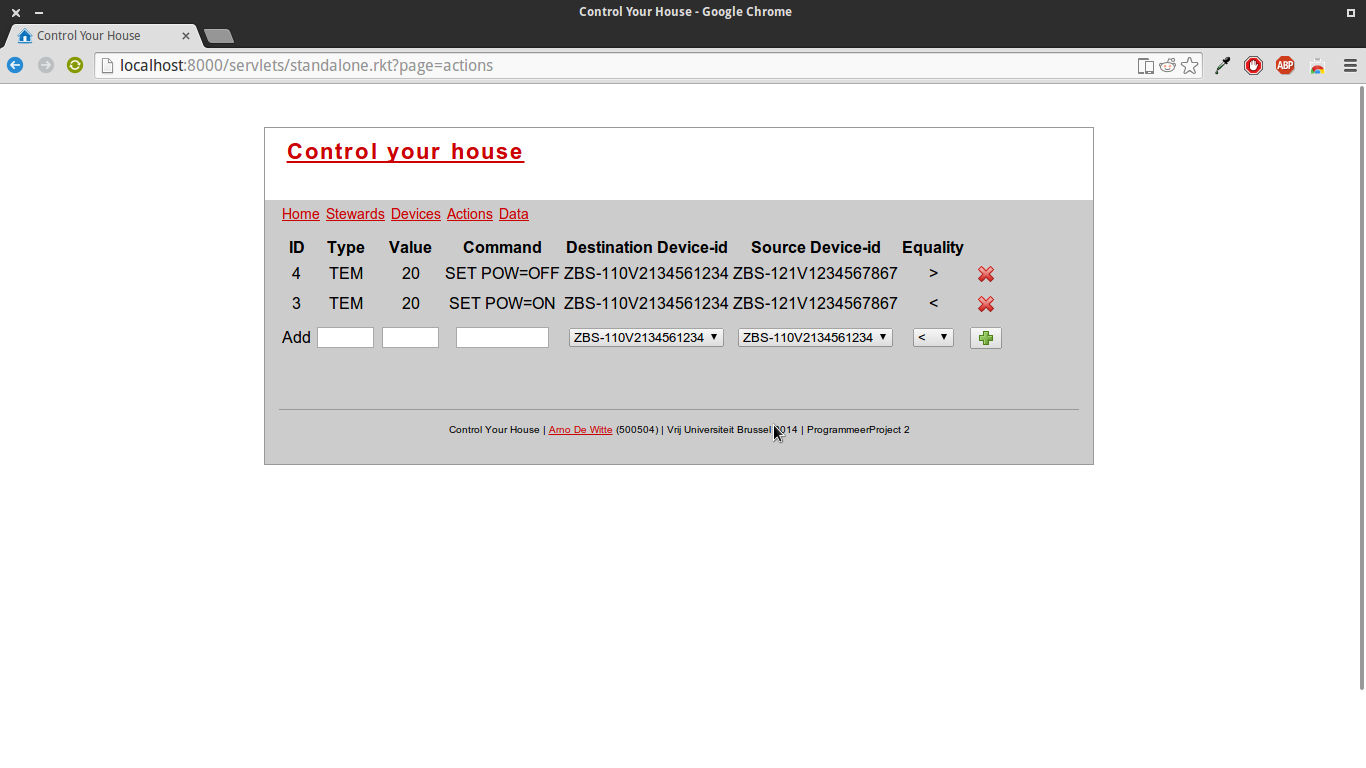
\includegraphics[scale=0.30]{Screenshot4.png}
\caption{Actie pagina}
\label{screen4}
\end{figure}
\begin{figure}[htp]
\centering
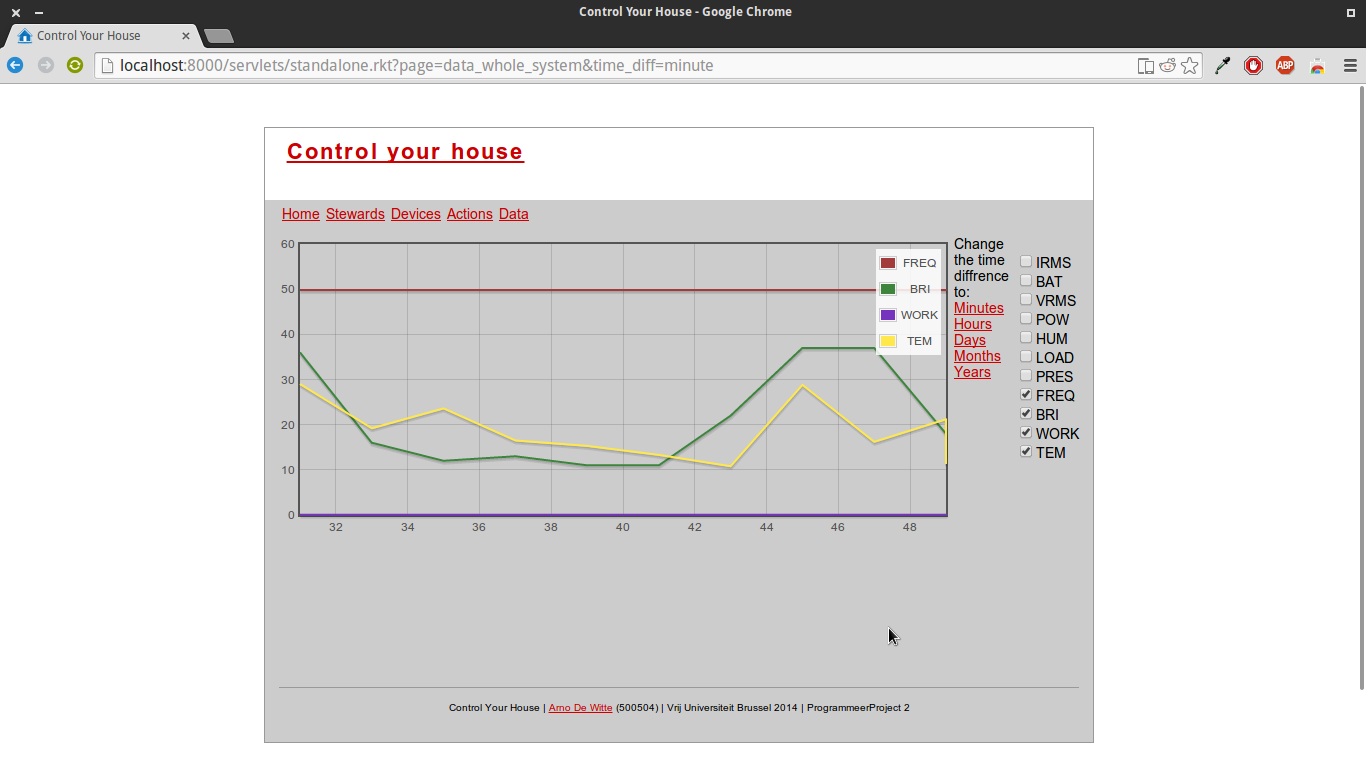
\includegraphics[scale=0.30]{Screenshot5.png}
\caption{Data grafiek}
\label{screen5}
\end{figure}
% subsection screenshots (end)

% section users (end)
\newpage

\section{Ontwikkelaars handleiding}
\label{sec:developers}
\subsection{Algemeen}
\label{sub:intro}
Hieronder volgt een beschrijving van het systeem voor ontwikkelaars. \\
Zoals eerder vermeld bestaat het systeem uit 3 verschillende pionnen. De majordomo (master genoemd), de stewards en de devices. De master is geschreven in racket en maakt gebruik van het klasse systeem dat bestaat in racket. Terwijl de steward geschreven is in slip een variatie van R5RS.\\
Er zijn enkele naming conventions in dit systeem. Eigenschappen van da objecten worden met een tilde geschreven. Bijvoorbeeld de master\ref{ssub:master} heeft als eigenschap een lijst met stewards. Deze wordt dan geschreven als $stewards\sim$.\\
Klassen worden genoteerd met een percent teken achter, bijvoorbeeld \emph{master\%}.\\
Omdat racket geen statische procedures ondersteunt (en alle publieke functies dus enkel kunnen worden opgeroepen met een instantie van een klasse), worden er waar nodig statische objecten aangemaakt. Dit zijn instanties van de klasse waar de data velden irrelevant zijn. Deze worden geschreven met een dollar teken achter. Bijvoorbeeld de statische variant van action wordt dan $action\$$.\\
\subsection{Klasse overzicht majordomo}
\label{sub:class}
Hieronder staat uitleg bij alle klassen die op de master draaien.
\subsubsection{Master}
\label{ssub:master}
Het kloppende hart van het systeem. Wanneer de klasse wordt aangemaakt moet de \textbf{init} procedure worden opgeroepen. Deze initialiseert de master, maakt een content-storer\ref{ssub:content-storer} en content-provider\ref{ssub:content-provider} klassen aan. Aan de content-provider gaat dan een lijst met stewards worden opgevraagd, deze worden op hun beurt dan ge\"initialiseerd. Verder vraagt het ook nog een lijst met acties op. Er worden ook 2 threads gestart. De eerste, save-thread, gaat na een bepaald interval de staat (stewards en devices) opslaan, dit gebeurt door de \textbf{save} procedure op te roepen. De andere gaat data verzamelen (statussen opvragen) en erna checken of er geen actions\ref{ssub:action} kunnen worden uitgevoerd. De procedures \textbf{collect-data} en \textbf{check-actions} zijn hier respectievelijk verantwoordelijk voor.\\
Verder heeft de master nog volgende procedures, deze worden veelal door de front-end\ref{ssub:front-end} aangesproken.
\begin{itemize}
	\item[get-all-rooms] geeft een lijst met alle kamers die in het systeem zitten terug. Deze worden opgeslagen in de database. Meer kamers kunnen worden in de settings bestand worden toegevoegd.
	\item[get-stewards] is een getter voor de stewards.
	\item[add-steward] voegt een nieuwe steward toe, gegeven een ip adres (in de vorm van een string) en een poort. Deze wordt dan aan de lijst toegevoegd. Er wordt ook save opgeroepen omdat we een aangepaste staat hebben.
	\item[get-steward] geeft het steward object terug voor een bepaald steward-id.
	\item[get-steward-for-device] geeft de steward terug die het device heeft dat bij een bepaald device-id hoort.
	\item[get-actions] geeft de lijst met actions terug.
	\item[add-action] voegt een actie object toe aan de lijst. Dit object wordt direct opgeslagen door de content-storer.
	\item[delete-action] gaat een action verwijderen. Er moet een id worden meegegeven. Deze wordt dan door de content-storer ook verwijderd uit de database.
	\item[check-actions] gaat alle acties na. Er wordt telkens de execute procedure opgeroepen met het passend steward object. Zo wordt nagegaan of de actie al dan niet moet worden uitgevoerd.
	\item[destruct] een destructor, deze gaat de threads be\"eindigen nadat een laatste keer de staat is gesaved.
	\item[get-facts] is een dispatch functies die verdeelt tussen verschillende feiten. Zoals bijvoorbeeld hoeveel data objecten er al zijn verzameld.
	\item[get-data] dient als tussen stuk tussen de front-end en de database met data objecten. 
\end{itemize}
% subsubsection master (end)

\subsubsection{Front end}
\label{ssub:front-end}
In dit data object wordt de interface geladen. Omdat we met een webinterface werken, wordt al de opmaak en styling gedaan in HTML en CSS. Er wordt gebruik gemaakt van het dynamische template systeem dat in racket zit\footnote{http://docs.racket-lang.org/web-server/templates.html}. Dit gaat html bestanden inlezen en wanneer het een @ tegenkomt wordt alles wat erachter komt ge\"evalueerd. Wanneer er bijvoorbeeld @variabele staat, zal dit vervangen worden door de waarde van de variabele. Er kunnen ook expressies worden meegegeven en ge\"itereerd worden over lijsten. De HTML template bestanden staan in de template map van het project. Het stijl bestand staat in de root van het project.\\
Om grafieken\footnote{http://www.flotcharts.org/} en een interactieve weergaven van berichten in  de interface te bekomen wordt er ook gebruik gemaakt van javascript en jQuery\footnote{http://jquery.com/}. Alle javascript libraries gebruikt in het project zijn te vinden in de js map. De gebruikte scripts (die zelf geschreven zijn) staan in de template bestanden waar ze worden toegepast.\\
Om aan te tonen dat de front-end kan worden uitgewisseld met bijvoorbeeld een front-end geschreven in racket GUI, is er een abstracte klasse front-end met een start procedure. Deze wordt in dit project dan ge\"implementeerd door html-front-end.\\
De belangrijkste procedure van deze klasse is \textbf{dispatche}. Deze neemt http requests en geeft responses terug. Dit gebeurt naargelang de aard van deze request. Bijvoorbeeld bij het opvragen van een pagina is er een GET request page met als waarde welke pagina er moet worden voorzien. \\
Bij kleinere calls, zoals voor de status, die via ajax worden gestuurd wordt rauwe data terug gestuurd. Maar bij pagina requests wordt heel de html pagina teruggegeven.\\ 
% subsubsection front-end (end)

\subsubsection{Database saveable}
\label{ssub:db-saveable}
Is een abstrace klasse die bepaalt welke procedures klassen moeten hebben om te kunnen worden opgeslagen in de database. Hieronder een kleine uitleg bij elk van deze procedures:
\begin{itemize}
		\item[store-sql] geeft de sql query terug die het object opslaagt. Dit in de vorm van een string. Omdat bij een insert het object zijn id moet weten of hij bij het opslaan ook andere objecten moet opslaan, kan er ook een conscel worden teruggegeven. In de car zit dan de sql en in de cdr een lambda procedure, deze neemt 2 argumenten: het id waarmee het ge\"insered is en de content-storer zodat het ook andere objecten kan opslaan.
		\item[get-sql] de select sql die nodig is om een object van dit type uit de database op te halen. Er moet wel nog een id worden achter geplakt. Dit is een statische procedure.
		\item[create-lambda] is de lambda die evenveel argumenten neemt als er velden wordt geselecteerd door de get-sql. Als resultaat geeft het een nieuw object van dit type terug. Natuurlijk is dit ook een statische procedure.
		\item[delete-sql] geeft de sql om de instatie van het object ter verwijderen uit de database.
\end{itemize}
% subsubsection db-saveable (end)

\subsubsection{Steward wrapper}
\label{ssub:steward}
Deze klasse is een abstractie van de echte steward. Dit wil zeggen dat het een racket object is. Maar dat de procedures geen effectieve berekeningen doen. De oproepen worden doorgestuurd naar de echte steward over het TCP/IP protocol.\\
De klassen implementeert de database-saveable klasse. Zo kunnen de stewards (die deel uitmaken van de staat van het systeem) persistent worden gemaakt. \\
De klasse heeft als eigenschappen: een lijst van device objecten, een ip en poort waarover de connectie verloopt, een plaats, een verwijzing naar het master object, input- en outputport die gebruikt wordt om berichten te sturen naar de effectieve steward, een status die zegt of de echte steward wel online is, een communication lock die ervoor zorgt dat de thread niet interfereert met andere communicatie en een variabele die zegt of er al eens is gezocht voor devices.\\
Bij het aanmaken van een instantie wordt er een thread ge\"initialiseerd, deze gaat in de achtergrond de devices en de status van elk device vragen. Deze wordt dan opgeslagen in respectievelijk dit object en het device object. Zo worden deze gegevens gecached.\\
Hieronder nog een bespreking van de overige noemsenwaardige procedures:
\begin{itemize}
  	\item[connect-to-pi] stelt de verbinding op over TCP/IP. Vult de waardes van de input en output porten maar ook van de status.
  	\item[send-mes-to-pi] is de private procedure die de messages over de output-port schrijft.
  	\item[get-device] geeft het juiste device object terug voor een gegeven device-id.
  	\item[online?] predicaat dat zegt of de steward online (en dus operationeel) is.
  	\item[get-device-count] zegt hoeveel devices er geconecteerd zijn aan deze steward.
  	\item[get-devices] geeft een lijst met device objecten terug. Deze lijst is gecached aan de hand van de thread.
  	\item[get-devices-force-discovery] gaat de devices effectief ophalen. Dit is de niet gecached versie.
  	\item[send-message-to-device] verstuurt een bericht naar een device. Deze effectief naar de fysieke devices gestuurt en dus niet lokaal naar het object.
  	\item[get-device-type] geeft het type van een device voor een bepaald device-id.
  	\item[get-device-status] geeft de gecached versie van de status terug. Deze wordt geparsed naar typed-data objecten. De status van een device is het  resultaat van een "GET" message.
  	\item[get-device-status-force-message] stuurt effectief de GET message om de status te bemachtigen.
  	\item[message-all-devices] stuurt een bericht naar alle devices.
  	\item[has-device?] predicaat dat zegt of een device verbonden is met deze steward.
\end{itemize}
% subsubsection steward (end)

\subsubsection{Device wrapper}
\label{ssub:device-wrapper}
Net zoals de bij de steward, is er een abstractie van de devices die op de majordomo zelf draait. Deze wrapper heeft minder procedures en wordt meer gebruikt om data over het device op te slaan. Het heeft alle eigenschappen die een echt device ook heeft: een communicatie adres waar berichten naar worden verzonden, een plek in het huis waar het zich bevindt, een type (bijvoorbeeld ZBS-110). Als extra eigenschappen heeft het ook een status, deze wordt gezet door de thread in de steward, een boolean die zegt of het device effectief gevonden is en een boolean die zegt of het device al is opgeslagen in de database.\\
Als procedures heeft het een serialize en deserialize procedure om het communicatie adres op te slaan. Er is echter een bug tussen racket en slip waardoor vectoren niet correct worden uitgelezen na een write over een output port. Hierdoor is het communicatie adres lokaal altijd null. Verder is er nog een procedure die het communicatie adres omzet in een leesbare string. Deze heeft met de bug ook niet veel nut.\\
Net zoals de steward wrapper, is de device wrapper ook een implementatie van database-saveable en kunnen devices (die een deel uitmaken van de staat van het systeem) ook worden opgeslagen in de database.
% subsubsection device-wrapper (end)

\subsubsection{Database manager}
\label{ssub:database-manager}
Deze klasse is verantwoordelijk voor het beheer van de database. Wanneer de database nog niet is ge\"initialiseerd gaat deze klasse hiervoor zorgen. Het handelt ook alle intereactie met de database af. Als database software is gebruik gemaakt van sqlite3\footnote{http://sqlite.org}. Racket voorziet hiervoor een interface binnen de taal\footnote{http://docs.racket-lang.org/db/}.\\
Het database bestand (sqlite slaat de database op in 1 bestand) is standaard \emph{./database/default} maar kan worden aangepast in het settingsbestand. De eigenschap install-query bevat een lijst met alle queries die worden gebruikt om de database aan te maken.
% subsubsection database-manager (end)

% subsection class (end)
% subsection intro (end)
% section developers (end)


\end{document}
